\documentclass[aps,prl,twocolumn,superscriptaddress,floatfix]{revtex4-2}

\usepackage[T1]{fontenc}
\usepackage{amsmath,amssymb,amsthm}
\usepackage{graphicx}
\usepackage{bm}
\usepackage{array}[=2016-10-06]
\usepackage{xcolor}
\definecolor{linkblue}{HTML}{1F5FBF}
\definecolor{citemagenta}{HTML}{C0157D}
\usepackage[colorlinks=true,linkcolor=linkblue,citecolor=citemagenta,urlcolor=linkblue]{hyperref}
\usepackage{orcidlink}
\hypersetup{pdftitle={The Fundamental Memory Ceiling of Noisy Quantum Reservoirs},pdfauthor={Markus Baumann, Jonas Stein, Claudia Linnhoff-Popien}}

\theoremstyle{plain}
\newtheorem{theorem}{Theorem}
\newtheorem{lemma}{Lemma}
\newtheorem{proposition}[lemma]{Proposition}
\newtheorem{corollary}[lemma]{Corollary}

\newcommand{\tr}{\operatorname{Tr}}
\newcommand{\ket}[1]{|#1\rangle}
\newcommand{\ketbra}[2]{|#1\rangle\!\langle #2|}
\newcommand{\nrm}[2]{\lvert #1\rvert_{#2}}
\newcommand{\Norm}[1]{\lVert #1\rVert}
\newcommand{\cD}{\mathcal D}
\newcommand{\cE}{\mathcal E}
\newcommand{\Nq}{\mathcal N_q}
\newcommand{\AD}{\mathcal{A\hspace{-0.6pt}D}}
\newcommand{\runin}[1]{\textit{\textbf{#1}}---}

\begin{document}

% The table of contents lists only the Supplemental Material: entries of the main text are not recorded.
\let\SMaddcontentsline\addcontentsline
\renewcommand{\addcontentsline}[3]{}

\title{The Fundamental Memory Ceiling of Noisy Quantum Reservoirs}

\author{Markus Baumann\,\orcidlink{0009-0007-3575-1006}}
\email[Contact author: ]{markus.baumann@campus.lmu.de}
\author{Jonas Stein\,\orcidlink{0000-0001-5727-9151}}
\author{Claudia Linnhoff-Popien\,\orcidlink{0000-0001-6284-9286}}
\affiliation{Quantum Applications and Research Laboratory (QAR-Lab),
Chair of Mobile and Distributed Systems, Department of Computer Science,
Ludwig-Maximilians-Universit\"at M\"unchen, Oettingenstra\ss e 67, 80538 M\"unchen, Germany}

\date{October 18, 2026}

\begin{abstract}
We show that enlarging a noisy quantum reservoir does not raise its fundamental memory ceiling. With $k$ input qubits reinitialized per time step, the longest memory any reservoir can attain under depolarizing noise is $\exp[\Theta(k)]$ time steps, whatever its size, dynamics, and input encoding. A universal upper bound and an explicit reservoir that attains the exponential scaling establish this optimal resource law. It extends to an entropy budget for general noise and applies to any noisy quantum dynamics refreshed by fresh qubits, including measurement-free error correction.
\end{abstract}

\maketitle

%======================================================================
% MAIN TEXT
%======================================================================

\runin{Introduction.}Reservoir computing processes time series with the transient dynamics of a fixed physical system, the reservoir: inputs are injected into it, and only a linear readout is trained~\cite{Jaeger2001,Maass2002,JaegerHaas2004,Lukosevicius2009,Tanaka2019}. Quantum reservoir computing (QRC) uses interacting qubits for this purpose~\cite{Fujii2017,Nakajima2019,Mujal2021} and has been realized on superconducting processors with up to 124 qubits~\cite{Chen2020,Suzuki2022,Yasuda2023,Hu2024,Monzani2024,Dao2026}. For temporal tasks, memory is the decisive resource. A reservoir that forecasts a time series can use an input only as long as that input still influences its state, and on noisy hardware this influence fades at every time step. Can a noisy quantum reservoir, or any noisy quantum system refreshed by fresh qubits [Fig.~\ref{fig:scope}], remember for arbitrarily long if it is only made large enough?

\begin{figure}[t]
\centering
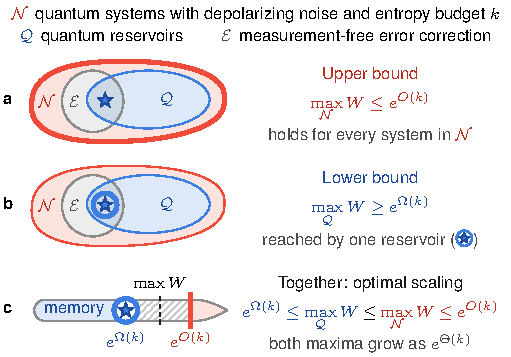
\includegraphics{fig1.pdf}
\caption{\textbf{Scope of the memory limit} (schematic).
(a)~The upper bound of Theorem~\ref{thm:main} holds for every system in $\mathcal N$, whatever its size and dynamics.
(b)~The lower bound is reached by one explicit reservoir (star): the error-correcting reservoir of Fig.~\ref{fig:attain}(a), which corrects errors without measurements.
(c)~On the memory axis, no system goes beyond the upper bound and the star reaches the lower bound, so the memory ceiling $\max W$ lies in between and grows as $e^{\Theta(k)}$ [Fig.~\ref{fig:limit}(b)].}
\label{fig:scope}
\end{figure}

\begin{figure*}[t]
\centering
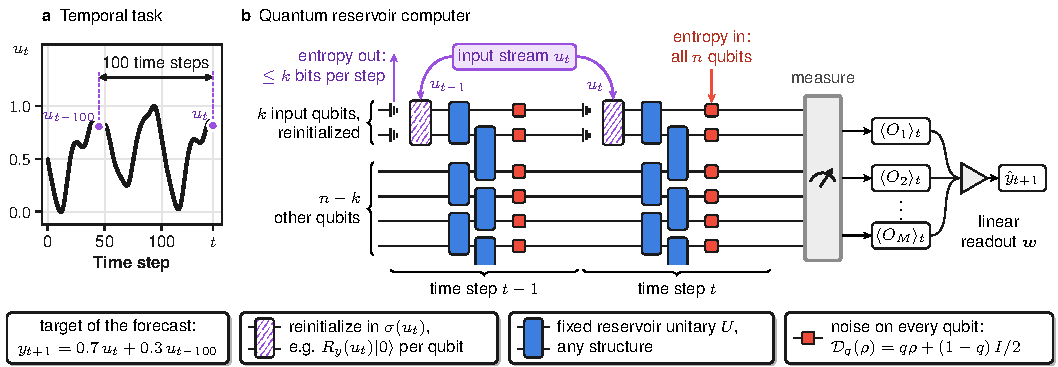
\includegraphics{fig2.pdf}
\caption{\textbf{Noisy quantum reservoir computing.}
(a)~Forecasting $y_{t+1}=0.7\,u_t+0.3\,u_{t-100}$ needs a memory of 100 time steps.
(b)~Every time step reinitializes $k$ input qubits in $\sigma(u_t)$, applies a fixed unitary $U$ to all $n$ qubits, and depolarizes every qubit; a linear readout predicts $\hat y_{t+1}$. Noise injects entropy into all $n$ qubits, but only the $k$ input qubits carry it out.}
\label{fig:overview}
\end{figure*}

The answer is not obvious. A larger reservoir offers more degrees of freedom in which to distribute information about past inputs, potentially making it more robust to noise. Yet redundancy alone does not prevent information from gradually degrading. Preserving it over long times may also depend on how the system is continually refreshed: in QRC, the input qubits are discarded and reinitialized at every time step, providing a route for removing accumulated entropy [Fig.~\ref{fig:overview}(b)]~\cite{Fujii2017,Yasuda2023,Hu2024}. Noise brings entropy into every qubit at every time step, whereas only the reinitialized qubits carry entropy out.

Echo-state and fading-memory criteria guarantee that old inputs eventually lose their influence~\cite{Jaeger2001,Boyd1985,MartinezPena2023,MorguiSancho2026}, Markovian reservoirs forget exponentially fast~\cite{Sannia2026}, and dissipation and resets are recognized resources for QRC~\cite{Chen2020,Kubota2023,Sannia2024,Monzani2024,Freiheit2026}. In noisy quantum computation, fresh qubits are known to be indispensable, since without them depolarizing noise permits only logarithmically deep computations~\cite{Aharonov1996,BenOr2013,StilckFranca2021,Mele2026}. How much memory a given supply of fresh qubits can buy has remained open.

Here we show that fresh qubits, not size, set a fundamental memory ceiling. Let $k$ input qubits be reinitialized at each time step, and let every qubit undergo depolarizing noise that keeps its state with probability $q$. The largest memory depth that any such reservoir can attain, that is, the number of past inputs that still influence its state beyond an accuracy $\varepsilon$, grows exponentially with $k$ and does not depend on the total number of qubits $n$ [Fig.~\ref{fig:limit}(b)]:
\begin{equation}
W_{q,k}(\varepsilon)=\exp\!\big[\Theta_q(k)\big].
\label{eq:main}
\end{equation}
This result is a fundamental resource limitation for an entire class of open quantum systems, not a property of a specific reservoir architecture [Fig.~\ref{fig:scope}], and three features make it physically significant. First, it is a universal no-go result: within a well-defined noise model, no architecture, however large and including ones not yet conceived, beats the dimension-independent upper bound, and an explicit reservoir attains its exponential dependence on the refresh budget $k$. Second, it identifies entropy removal as the resource that limits memory: memory is bought with reinitialized qubits, not with size, and retaining an input for $T$ time steps requires, and can be achieved with, $\Theta_q(\log T)$ reinitialized qubits per time step [Fig.~\ref{fig:limit}(a)]. Third, it governs the stabilization of information in noisy quantum systems in general: the proof uses only the entropy budget of each noisy time step, so the law applies to any noisy quantum dynamics refreshed by fresh qubits without classical feedback, from dynamical circuits with resets~\cite{Yasuda2023,Hu2024} to measurement-free error correction~\cite{Heussen2024}, and complements space-overhead bounds for fault-tolerant quantum computation~\cite{Fawzi2022}.

Our explicit error-correcting reservoir shows how fresh qubits sustain long memory under depolarizing noise. Its fixed dynamics protects the stored information while transferring accumulated entropy to the input register, where it is removed at the next reinitialization. The resulting memory depth grows exponentially with the number of reinitialized input qubits, realizing the optimal scaling established by our bounds.

\runin{A reservoir with fresh qubits.}A reservoir of $n$ qubits receives one classical input $u_t$ per time step $t$ [Fig.~\ref{fig:overview}(a),(b)]. At each time step, the $k$ qubits of the input register are discarded and reinitialized in an input state $\sigma(u_t)$ that encodes the input. A fixed reservoir unitary $U$ then acts on all qubits. Finally, every qubit undergoes depolarizing noise $\cD_q(\rho)=q\rho+(1-q)\tr(\rho)I/2$. Altogether,
\begin{equation}
\rho_t=\cD_q^{\otimes n}\Bigl(U\bigl[\sigma(u_t)\otimes\tr_{\mathrm{in}}\rho_{t-1}\bigr]U^\dagger\Bigr),
\label{eq:model}
\end{equation}
where $\tr_{\mathrm{in}}$ is the partial trace over the input register. A trained linear readout turns the state into a prediction $\hat y_{t+1}=\sum_iw_i\tr(O_i\rho_t)=\tr(F\rho_t)$. This covers the original QRC proposal~\cite{Fujii2017} and protocols that measure and reset qubits without feedback~\cite{Yasuda2023,Hu2024}. We impose no restriction on $\sigma(u)$ or $U$; the unitary may even depend on the input.

The input qubits enter our analysis through a single number. Because $\sigma(u)\le I$, one time step can lower the entropy of a completely mixed reservoir by at most $k$ bits; formally, the map $\cE_u(X)=U[\sigma(u)\otimes\tr_{\mathrm{in}}X]U^\dagger$ obeys $\cE_u(I)\le2^kI$. We call $k$ the entropy \emph{budget} of a time step. It is the only property of the input injection that the upper bound uses.

Noise erases the initial state, so the reservoir eventually reaches a state that depends only on the input history $h=(\dots,u_{t-1},u_t)$, its \emph{echo state} $\rho(h)$~\cite{Jaeger2001,MartinezPena2023,SM}. The \emph{memory depth} $W(\varepsilon)$ is the smallest number $L$ of time steps such that any two input histories that agree on their last $L$ inputs lead to echo states with
\begin{equation}
\tfrac12\Norm{\rho(h)-\rho(h')}_1\le\varepsilon .
\label{eq:depth}
\end{equation}
Inputs older than $W(\varepsilon)$ change every linear readout by at most $2\varepsilon\Norm F$~\cite{SM}: unlike the memory capacity~\cite{Jaeger2002}, the memory depth limits all readouts at once. We write $W_{q,k}(\varepsilon)$ for the largest memory depth of any reservoir with $k$ input qubits, maximized over $n$, $U$, and $\sigma$.

\begin{figure*}[t]
\centering
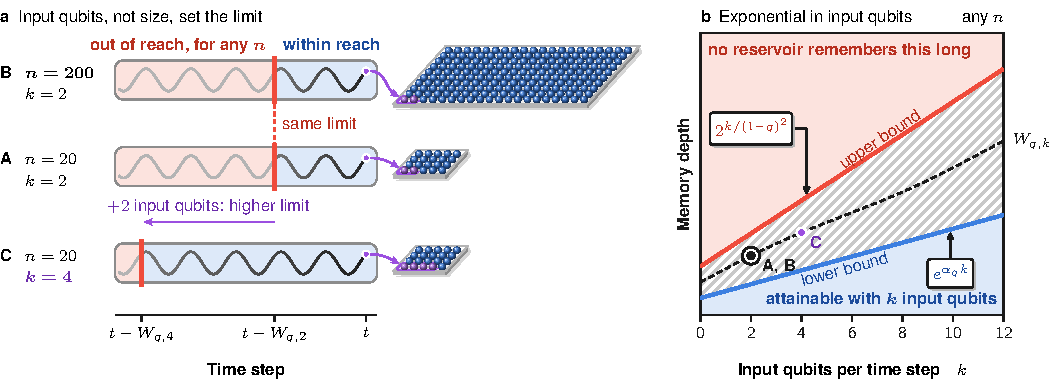
\includegraphics{fig3.pdf}
\caption{\textbf{The memory limit} (schematic).
(a)~One input stream drives A and B, which differ tenfold in size but share $k=2$ input qubits, and C, which is A with two more. Inputs older than the limit (red) are out of reach for every reservoir with the same $k$: A and B share the limit $W_{q,2}$, and C has a higher attainable limit.
(b)~The limit lies between two exponentials in $k$, for every $n$ (Theorem~\ref{thm:main}); A, B, and C as in (a).}
\label{fig:limit}
\end{figure*}

\runin{The memory limit.}Our main result bounds $W_{q,k}$ from both sides.

\begin{theorem}[Memory limit]\label{thm:main}
Let $0<q<1$ and $0<\varepsilon<q$.\\[2pt]
(i)~Every reservoir with $k\ge4$ input qubits has
\begin{equation}
W(\varepsilon)\le\Bigl\lceil2^{k/(1-q)^2}\ln\frac1\varepsilon\Bigr\rceil,
\label{eq:upper}
\end{equation}
whatever its number of qubits, reservoir unitary, and input encoding.\\[2pt]
(ii)~For every $k$ with $e^{\alpha_q(k-3)}\ge4$, where $\alpha_q=\frac12\ln\frac1{1-q^2}$, some reservoir with at most $2k$ qubits has
\begin{equation}
W(\varepsilon)\ge\tfrac14\,e^{\alpha_q(k-3)}\ln\frac q\varepsilon .
\label{eq:lower}
\end{equation}
\end{theorem}

Theorem~\ref{thm:main} characterizes the optimal resource scaling over the entire class of admissible reservoirs, not the performance of a particular architecture: the upper bound holds for every member, and the lower bound is an existence result, reached by one explicit member [Fig.~\ref{fig:scope}]. Since the two exponents differ, the theorem fixes the scaling class, not the exact rate [Fig.~\ref{fig:limit}(b)]. For $k\le3$, the upper bound holds with $k+1$ in place of $k$~\cite{SM}.

The theorem concerns echo states: $n$ redundant copies of an initial bit take $\Theta_q(\log n)$ time steps to wash out~\cite{SM}, so a larger reservoir needs a longer washout but does not remember new inputs for longer. Its constants are conservative~\cite{SM}; it identifies the resource and its scaling.

\runin{Why no reservoir can remember longer.}A proof must defeat every strategy a reservoir might use to hide information: spreading it over many qubits, entangling it, or using its input qubits for repair. Our proof follows the difference between two reservoir states with different input histories and asks how well the states can be distinguished and how concentrated their difference is on a small part of the Hilbert space. Two established properties of depolarizing noise answer these questions~\cite{King2014,Cubitt2015} and yield the bound in three steps.

\emph{Step 1: Noise caps the purity.} We measure the purity of a state by $\log_2P^2=n-S_2(\rho)$, the number of pure qubits' worth of purity it holds, where $S_2$ is the R\'enyi-2 entropy. Depolarizing noise damps the many-qubit correlations of which purity is made, a property known as hypercontractivity~\cite{King2014}. As a result, every time step multiplies the log-purity by $\theta=2q^2/(1+q^2)<1$, while the input qubits add at most $\theta k$. The log-purity thus has a fading memory of its own, and whatever its size, every echo state holds at most $\log_2P_*^2=2kq^2/(1-q^2)$ pure qubits' worth of purity, about 8.5 per input qubit at $q=0.9$~\cite{SM}.

\emph{Step 2: Spread-out differences are erased.} Low purity alone does not mean forgetting: $\ketbra00\otimes I/2^{n-1}$ and $\ketbra11\otimes I/2^{n-1}$ are almost completely mixed, yet perfectly distinguishable. Their difference, however, is spread over the whole Hilbert space, and one layer of noise erases the fraction $1-q$ of their distinguishability. A difference survives noise only if it is concentrated on a small subspace, as for a bit stored in many redundant copies. Reverse hypercontractivity makes this precise~\cite{Cubitt2015}: noise forces two states to overlap unless their difference is concentrated, so one layer of noise erases a fixed fraction of every spread-out difference.

\emph{Step 3: Concentration costs purity.} A distinguishable difference concentrated on a fraction $2^{-m}$ of the Hilbert space, such as a bit stored in $m$ redundant copies, requires about $m$ pure qubits' worth of purity, and Step~1 caps the purity. A distance $V$ that weighs distinguishability against concentration~\cite{SM} therefore shrinks at every time step $\Phi_u$, for any two reservoir states $\rho,\rho'$ and any input $u$:
\begin{equation}
V\bigl(\Phi_u\rho-\Phi_u\rho'\bigr)\le(1-\delta)\,V(\rho-\rho'),
\label{eq:contraction}
\end{equation}
with a forgetting rate $\delta\ge2^{-k/(1-q)^2}$ for $k\ge4$~\cite{SM}. Whatever the reservoir does, every time step erases at least the fraction $\delta$ of its past. After $L$ time steps, two echo states are therefore within trace distance $e^{-\delta L}$, which is Theorem~\ref{thm:main}(i).

Without fresh qubits, $k=0$, as for inputs encoded in input-dependent unitaries, the echo state is the completely mixed state for every input sequence: such a reservoir retains nothing.

\begin{figure*}[t]
\centering
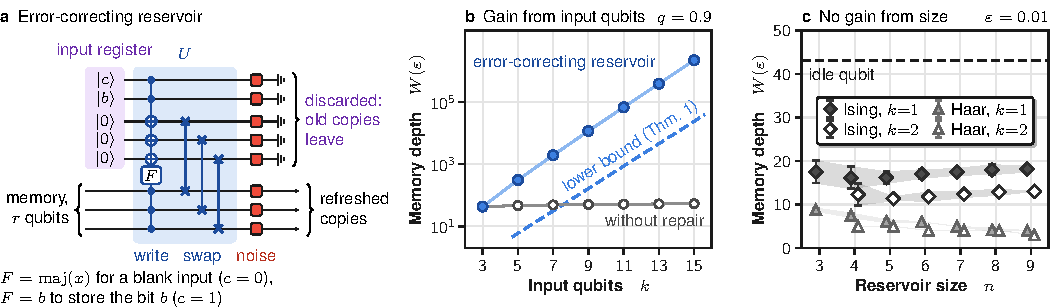
\includegraphics{fig4.pdf}
\caption{\textbf{Attaining the limit.}
(a)~Error-correcting reservoir ($r=3$, $k=5$): $U$ writes the new bit, or the majority of the stored copies, into fresh ancillas and swaps them into the memory; the old copies leave with the input register.
(b)~The error-correcting reservoir (exact single-qubit readout, $n=2k-2$) uses its fresh qubits for repair, and its memory depth grows exponentially with $k$, above the lower bound of Theorem~\ref{thm:main}; without repair, the same $r=k-2$ copies gain almost nothing, even with the best readout. Depths with and without repair are plotted at continuous threshold crossings; the corresponding integer depths are rounded up.
(c)~Within the sampled ensembles, standard reservoirs gain nothing from size, and a second input qubit shortens their memory ($k=1$ filled, $k=2$ open; mean $\pm$ s.d., six realizations). Unitaries are sampled separately for each $k$. (b),~(c)~$q=0.9$, $\varepsilon=0.01$.}
\label{fig:attain}
\end{figure*}

\runin{A reservoir that attains the limit.}Because $W_{q,k}$ is an optimum over all admissible reservoirs, a single reservoir suffices to show that the exponential scaling is attained. We deliberately choose the simplest one whose dynamics is exactly solvable; its role is to show that the exponential dependence on $k$ is fundamental rather than an artifact of the upper-bound proof.

The idea is a memory that repairs itself with fresh qubits, an error-correcting reservoir [Fig.~\ref{fig:attain}(a)]. It stores a bit in $r$ memory qubits as a repetition code and corrects it by majority vote: at every time step, its unitary computes the majority of the stored copies, writes it into $r$ freshly reinitialized ancillas, and swaps the ancillas into the memory. The old copies, which carry the noise of the previous time step, end up in the input register and are discarded at the next injection, so the entropy leaves with them. Two further input qubits tell the reservoir whether to keep its memory or to store a new bit, so that $k=r+2$~\cite{SM}. The unitary only permutes computational basis states, so the reservoir corrects errors without measurements or feedback.

Because all states remain diagonal, every qubit behaves as a classical bit that flips with probability $(1-q)/2$ per time step, and the response can be computed exactly. The stored bit is lost only if most of its $r$ copies flip within one time step, which happens with probability $p_r\le(1-q^2)^{r/2}=e^{-\alpha_qr}$ by a Chernoff bound with the exact exponent~\cite{SM}. A bit $b$ stored $t$ time steps ago therefore yields on any memory qubit
\begin{equation}
\langle Z\rangle_t=(-1)^b\,q\,(1-2p_r)^t .
\label{eq:response}
\end{equation}
The signal still decays, but at a rate that is exponentially small in $r$. Two input histories that differ only in this bit agree on their last $t$ inputs, yet their echo states remain at trace distance at least $q(1-2p_r)^t$; with the bound on $p_r$, this gives Theorem~\ref{thm:main}(ii). At $q=0.9$ and $\varepsilon=0.01$, the memory depth exceeds 300 time steps for $k=5$ and two million for $k=15$, whereas the same copies without the majority vote keep the bit for at most 53 time steps [Fig.~\ref{fig:attain}(b)].

\runin{Standard reservoirs operate far below the limit.}We simulated transverse-field Ising reservoirs with random all-to-all couplings, the workhorse of QRC~\cite{Fujii2017,Nakajima2019,MartinezPena2021}, and Haar-random unitaries at $q=0.9$, and estimated their memory depth $W$ at $\varepsilon=0.01$ from input histories that differ in one input or in all earlier inputs~\cite{SM}. Within these ensembles, size does not extend their memory [Fig.~\ref{fig:attain}(c)]: with one input qubit ($k=1$), the Ising reservoir remembers 16 to 18 time steps for every size from $n=3$ to $9$ qubits, and the Haar reservoir forgets faster as it grows ($W$ drops from 9 to 4 time steps as $n$ grows from 3 to 9). More input qubits do not help either [Fig.~\ref{fig:attain}(c)]~\cite{SM}: at fixed size ($n=8$), raising $k$ from 1 to 4 lowers $W$ from 18 to 8 time steps (Ising) and from 4 to 3 (Haar); the decrease persists when the additional input qubits are reinitialized in $\ket0$. Both stay below an idle qubit that merely holds the input ($W=43$ time steps), whereas the error-correcting reservoir of the same size ($n=8$, of which $k=5$ are input qubits) remembers 316 time steps.

\runin{An entropy budget.}Beyond depolarizing noise, the result becomes an entropy budget~\cite{SM}: any additional channel $\mathcal S$ with $\mathcal S(I)\le2^bI$ adds $b$ bits, and the upper bound holds with $k$ replaced by $k+b$. Unital noise (Pauli errors, dephasing, coherent errors, crosstalk) and projective measurements whose outcomes only enter the readout~\cite{Mujal2023} have $b=0$; since every unital qubit channel with full-rank Choi matrix contains a depolarizing component, the theorem covers generic independent unital noise~\cite{SM}. Resets of $m$ qubits count like $m$ input qubits. Amplitude damping with probability $0<\gamma<1$ adds $n\log_2(1+\gamma)$ bits, and relaxing idle qubits then act as a refrigerator~\cite{BenOr2013} that lets a reservoir with two input qubits remember for a time exponential in $n$~\cite{SM,Hoeffding1963}. Without a depolarizing component, with non-Markovian noise~\cite{Sannia2026}, or with feedback of measurement outcomes, memory can be unbounded~\cite{SM}.

\runin{Conclusion.}Fresh qubits, not size, set the memory of noisy quantum reservoirs. A dimension-independent upper bound for arbitrary dynamics and an explicit reservoir that attains its exponential scaling establish an optimal resource law and a universal no-go result for an entire class of open quantum systems, from QRC to measurement-free error correction~\cite{Heussen2024}: with $k$ reinitialized qubits per time step, the memory ceiling is $\exp[\Theta_q(k)]$ time steps, whatever the size. Fresh qubits are necessary to reach the ceiling but not sufficient; standard reservoirs, which do not use them for repair, operate far below it. When a reservoir forgets too quickly, the parameters to check are therefore its supply of fresh qubits and whether its dynamics uses them to remove errors, not its size. The theorem bounds how far back any task can reach, not how well a reservoir processes the inputs within that range~\cite{Cao2026}. Open problems include closing the gap between the two exponents, extending the bound to feedback and non-Markovian noise, and testing the scaling by varying $k$ at fixed $n$ with mid-circuit resets~\cite{Yasuda2023,Hu2024}.

\begin{acknowledgments}
\runin{Acknowledgments.}Markus Baumann used Claude Opus 5.5 (Anthropic) to assist with drafting and editing the text, checking derivations and references, and writing the simulation and plotting code. Markus Baumann directed this work, verified every derivation and numerical result, and takes full responsibility for the content of this article.
\end{acknowledgments}

\runin{Data availability.}Code and data that reproduce all numbers and figures of this Letter are provided as a source archive with the Supplemental Material~\cite{SM}.

% References cited only in the Supplemental Material (through the note of Ref. SM); the \nocite lets a single
% BibTeX run of the Letter alone find them, with the same numbering.
\nocite{vonNeumann1956,Nelson2026,Xiong2025}
\bibliography{refs}

\end{document}
